\documentclass[../../../../main.tex]{subfiles}

\begin{document}

\section*{第1問}

\begin{proof}[解]
(1) $f'(x) = n x^{n-1}$ と、$f(x)$ が偶関数あるいは奇関数なことより、$|f(x)| < \frac{1}{1000} \quad \left(-\frac{1}{2} \le x \le \frac{1}{2}\right)$ を満たすには
\[
\left| f\left(\frac{1}{2}\right) \right| < \frac{1}{1000}
\]
であれば良い. 代入して
\[
\left(\frac{1}{2}\right)^n < \frac{1}{1000} \quad \cdots \text{①}
\]
ここで、$2^{10} = 1024 > 1000$ から $\left(\frac{1}{2}\right)^{10} < \frac{1}{1000}$. 同様に $\left(\frac{1}{2}\right)^9 > \frac{1}{1000}$ だから ①をみたす $n$ は $n \ge 10$ である ($y = \left(\frac{1}{2}\right)^x$ は $x>0$ で単調減少).

\medskip
(2) (1)で $x = \frac{X}{2}$ とおきかえると、$f(x) = \left(\frac{1}{2}\right)^n X^n \ (n \ge 10)$ は $-1 \le X \le 1$ で $|f(x)| < \frac{1}{1000}$ をみたす. そこで $g(x) = \left(\frac{1}{2}\right)^n x^n$ とおき、$10 \le n \in \mathbb{N}$ のうちで
\[
10^4 < g(3) < 10^5 \quad \cdots \text{②}
\]
であるような $n$ をさがす.

ところで、
\[
\left(\frac{3}{2}\right)^{11} \le 10^2 \quad (\because 3^5 = 243, \, 2^5 \cdot 10 = 320)
\]
\[
\left(\frac{3}{2}\right)^6 \ge 10 \quad (\because 3^6 - 2^6 \cdot 10 = 829 - 640 > 0)
\]
の両辺 $\log_{10}$ をとって
\[
6 > \frac{1}{\log_{10} \frac{3}{2}} \ge \frac{11}{2} \quad \cdots \text{③}
\]
さらに、②の両辺 $\log_{10}$ をとって
\[
4 < n \log_{10} \frac{3}{2} < 5 \quad \cdots \text{④}
\]
$\log_{10} \frac{3}{2} > 0$ から、
\[
\frac{4}{\log_{10} \frac{3}{2}} < n < \frac{5}{\log_{10} \frac{3}{2}} \quad \cdots \text{⑤}
\]
④をみたすような $n$ は②を満たし、④から⑤を満たす $n$ は
\[
24 > \frac{4}{1/6} < n < \frac{5}{1/5.5} = \frac{55}{2} = 27.5
\]
もみたす. したがって、たとえば $n = 25$ とした $g(x) = \left(\frac{x}{2}\right)^{25}$ は解の1つ ($\because 25 \ge 10$).
\end{proof}

\begin{proof}[別解]
(1)から $g(x) = f(x - 1/2) = (x - 1/2)^n \ (n \ge 10)$ とすると前半の条件を満たす.
\end{proof}

\newpage

\section*{第2問}

\begin{proof}[解]
(1) $S$ のベクトル $\vec{a}, \vec{b}$ のなす角を $\theta$ とすると ($0 \le \theta \le \pi$), 条件から
\[
2 \frac{|\vec{a}|}{|\vec{b}|} \cos\theta \in \mathbb{Z}
\]
又、$\vec{a}, \vec{b}$ を逆にした
\[
2 \frac{|\vec{b}|}{|\vec{a}|} \cos\theta \in \mathbb{Z}
\]
も成り立ち、したがって、辺々かけあわせて
\[
4 \cos^2\theta \in \mathbb{Z} \quad \cdots \text{①}
\]
$0 \le \cos^2\theta \le 1$ だから、①がみたされるのは
\[
4 \cos^2\theta = 0, 1, 2, 3, 4
\]
\[
\iff \cos^2\theta = 0, \frac{1}{4}, \frac{1}{2}, \frac{3}{4}, 1
\]
\[
\iff \cos\theta = 0, \pm \frac{1}{2}, \pm \frac{1}{\sqrt{2}}, \pm \frac{\sqrt{3}}{2}, \pm 1
\]
\[
\iff \theta = 0, \frac{\pi}{6}, \frac{\pi}{4}, \frac{\pi}{3}, \frac{\pi}{2}, \frac{2}{3}\pi, \frac{3}{4}\pi, \frac{5}{6}\pi, \pi
\]
より題意は示された.

\medskip
(2) 角が $0$ の時. $2 \frac{|\vec{a}|}{|\vec{b}|}, 2 \frac{|\vec{b}|}{|\vec{a}|} \in \mathbb{Z}$ から,
\[
2 \frac{|\vec{a}|}{|\vec{b}|} = k, \quad 2 \frac{|\vec{b}|}{|\vec{a}|} = m \quad (k, m \in \mathbb{N})
\]
とおける. 辺々かけあわせて $4 = km$ より $(k, m) = (1, 4), (2, 2), (4, 1)$ だが、このうち $|\vec{a}| = |\vec{b}| \iff k = 2 = m$ を満たすのは $k=1, 2$ の時で
\[
|\vec{a}| : |\vec{b}| = 1 : 1, \quad 1 : 2
\]
・角が $\pi/6$ の時, 同様に $k, m \in \mathbb{N}$ として
\[
\sqrt{3} \frac{|\vec{a}|}{|\vec{b}|} = k, \quad \sqrt{3} \frac{|\vec{b}|}{|\vec{a}|} = m
\]
辺々かけて $3 = km$ より $(k, m) = (1, 3), (3, 1)$. これらは $|\vec{a}| : |\vec{b}| = k : \sqrt{3} = \sqrt{3} : m$ をみたすから、2ベクトルの比は $1 : \sqrt{3}$.

・角が $\pi/3$ の時, $\frac{|\vec{a}|}{|\vec{b}|}, \frac{|\vec{b}|}{|\vec{a}|} \in \mathbb{Z}$ から ベクトルの比は $1 : 1$.

\medskip
(3) まず, $\vec{a} = \begin{pmatrix} 1 \\ 0 \end{pmatrix}, \vec{b} = |\vec{b}| \begin{pmatrix} \cos \pi/6 \\ \sin \pi/6 \end{pmatrix}$ とおける. なす角が $120^\circ, 150^\circ$ の時の2ベクトルの比は (2)の $60^\circ, 30^\circ$ の場合に等しく, $90^\circ$ の時は鏡であることから、下図のようにとればこれらは集合 $S$ になる. (ただし片方のベクトルのなす角 $30^\circ$)

\begin{center}
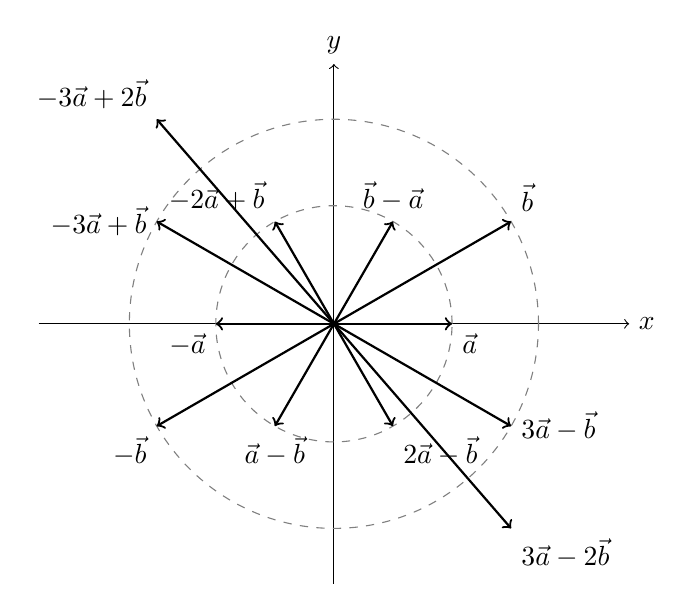
\begin{tikzpicture}[scale=1.5]
  \draw[->] (-2.5,0) -- (2.5,0) node[right] {$x$};
  \draw[->] (0,-2.2) -- (0,2.2) node[above] {$y$};
  \draw[dashed, gray] (0,0) circle (1);
  \draw[dashed, gray] (0,0) circle (1.732);
  
  % Rays / Vectors
  \draw[->, thick] (0,0) -- (1,0) node[below right] {$\vec{a}$};
  \draw[->, thick] (0,0) -- (1.5, 0.866) node[above right] {$\vec{b}$};
  \draw[->, thick] (0,0) -- (0.5, 0.866) node[above] {$\vec{b}-\vec{a}$};
  \draw[->, thick] (0,0) -- (-1.5, 1.732) node[above left] {$-3\vec{a}+2\vec{b}$};
  \draw[->, thick] (0,0) -- (-0.5, 0.866) node[above left] {$-2\vec{a}+\vec{b}$};
  \draw[->, thick] (0,0) -- (-1.5, 0.866) node[left] {$-3\vec{a}+\vec{b}$};
  \draw[->, thick] (0,0) -- (-1,0) node[below left] {$-\vec{a}$};
  \draw[->, thick] (0,0) -- (-1.5, -0.866) node[below left] {$-\vec{b}$};
  \draw[->, thick] (0,0) -- (-0.5, -0.866) node[below] {$\vec{a}-\vec{b}$};
  \draw[->, thick] (0,0) -- (1.5, -1.732) node[below right] {$3\vec{a}-2\vec{b}$};
  \draw[->, thick] (0,0) -- (0.5, -0.866) node[below right] {$2\vec{a}-\vec{b}$};
  \draw[->, thick] (0,0) -- (1.5, -0.866) node[right] {$3\vec{a}-\vec{b}$};
\end{tikzpicture}
\end{center}

これらを $\vec{a}, \vec{b}$ で表すと、$\vec{a}, \vec{b}$ から反時計回りに順に
\[
\vec{a}, \, \vec{b}, \, \vec{b}-\vec{a}, \, -3\vec{a}+2\vec{b}, \, -2\vec{a}+\vec{b}, \, -3\vec{a}+\vec{b}, \, -\vec{a}, \, -\vec{b}, \, \vec{a}-\vec{b}, \, 3\vec{a}-2\vec{b}, \, 2\vec{a}-\vec{b}, \, 3\vec{a}-\vec{b}
\]
\end{proof}

\newpage

\section*{第3問}

\begin{proof}[解]
$f(x)$ の最高次を $a_n x^n \ (a_n \ne 0, n \in \mathbb{Z}_{\ge 0})$ とおくと,
$f(x) \cdot f'(x)$ の最高次は $n a_n^2 x^{2n-1}$, $\int_0^x f(t) dt$ の最高次は $\frac{a_n}{n+1} x^{n+1}$ である.

\medskip
$1^\circ \ n \ge 3$ の時\\
$2n-1 > n+1$ から、与式左辺の最高次は $n a_n^2 x^{2n-1}$ だから 比較して
\[
n \cdot a_n^2 \cdot x^{2n-1} = \frac{4}{9} x
\]
しかしこれをみたす $n \in \mathbb{N}_{\ge 3}$ は存在せず、不適.

\medskip
$2^\circ \ n \le 1$ の時\\
$2n-1 < n+1$ から、$1^\circ$ と同様にして
\[
\frac{a_n}{n+1} x^{n+1} = \frac{4}{9} x
\]
より、$(a_n, n) = \left(\frac{4}{9}, 0\right)$, つまり $f(x) = \frac{4}{9}$ が必要. 与式に代入して
\[
(\text{左辺}) = \frac{4}{9} (x - 1)
\]
となり、十分.

\medskip
$3^\circ \ n = 2$ の時\\
この時、$n a_n^2 + \frac{a_n}{n+1} \ne 0$ の時、与式左辺の最高次は $x^3$ となり矛盾. 従って $n a_n^2 + \frac{a_n}{n+1} = 0$ が必要で、$n=2, a_n \ne 0$ とあわせて $a_n = -\frac{1}{6}$ だから、$f(x) = -\frac{1}{6} x^2 + ax + b$ とおける. 代入して
\[
\left( -\frac{1}{6} x^2 + ax + b \right) \left( -\frac{1}{3} x + a \right) = \frac{1}{18} x^3 + \frac{a}{2} x^2 + bx + \frac{1}{18} - \frac{a}{2} - b = \frac{4}{9} (x - 1)
\]
\[
\left( a^2 + \frac{2}{3} b \right) x + ab - \frac{1}{2} a - b + \frac{1}{18} = \frac{4}{9} (x - 1)
\]
係数比較して
\[
a^2 + \frac{2}{3} b = \frac{4}{9} \quad \cdots \text{①}
\]
\[
(a - 1) b - \frac{1}{2} a + \frac{1}{18} = -\frac{4}{9} \quad \cdots \text{②}
\]
①を②に代入整理して $(a-1)\left(\frac{1}{2} - a^2\right) = 0$ だから、
$(a, b) = \left(1, -\frac{5}{6}\right), \left(\pm \frac{1}{\sqrt{2}}, \frac{1}{6}\right)$ だから、
\[
f(x) = -\frac{1}{6} x^2 + x - \frac{5}{6}, \quad -\frac{1}{6} x^2 \pm \frac{1}{\sqrt{2}} x + \frac{1}{6}
\]

以上から
\[
f(x) = \frac{4}{9}, \quad -\frac{1}{6} x^2 + x - \frac{5}{6}, \quad -\frac{1}{6} x^2 \pm \frac{\sqrt{2}}{2} x + \frac{1}{6}
\]
\end{proof}

\newpage

\section*{第4問}

\begin{proof}[解]
$a_n > 0$
\[
a_n^3 + 3 a_n^2 - \left(9 + \frac{1}{n}\right) a_n + 5 < 0 \quad \cdots \text{①}
\]
①を変形して
\[
(a_n - 1)^2 < \frac{1}{n} \frac{a_n}{a_n + 5} \quad (\because a_n > 0) \quad \cdots \text{②}
\]
又、$f_n(x) = x^3 + 3x^2 - \left(9 + \frac{1}{n}\right) x + 5$ とおくと
\[
f_n'(x) = 3x^2 + 6x - \left(9 + \frac{1}{n}\right)
\]
より、$f_n'(x) = 0$ の2根 $\alpha, \beta \ (\alpha < \beta)$ として下表を与える.

\begin{center}
\begin{tabular}{c|ccccc}
$x$ & $\dots$ & $\alpha$ & $\dots$ & $\beta$ & $\dots$ \\ \hline
$f_n'$ & $+$ & $0$ & $-$ & $0$ & $+$ \\ \hline
$f_n$ & $\nearrow$ & & $\searrow$ & & $\nearrow$
\end{tabular}
\end{center}

\begin{center}
\begin{tikzpicture}[scale=0.8]
  \draw[->] (-3,0) -- (3,0) node[right] {$x$};
  \draw[->] (0,-4) -- (0,6) node[above] {$y$};
  \draw[domain=-2.8:1.8, smooth, variable=\x, blue, thick] plot ({\x}, {\x*\x*\x + 3*\x*\x - 9.1*\x + 5});
  \node[above left] at (-2.1, 15) {};
  \draw[dashed] (1.1, 0) node[below] {$\beta$} -- (1.1, -1.8);
  \draw[dashed] (-3.1, 0) node[above] {$\alpha$} -- (-3.1, 20);
  \node[right] at (1.1, -1.8) {$(\beta = -1 + \sqrt{4 + \frac{1}{3n}})$};
\end{tikzpicture}
\end{center}

従ってグラフは右上図のようになる. から、$\beta < x$ では $x$ は単調増加, $0 < x < \beta$ では $x$ は単調減少である. よって明らかに $0 < a_n < \frac{5}{3}$.

$y = \frac{x}{x+5}$ のグラフを考えてこの時

\begin{center}
\begin{tikzpicture}[scale=0.8]
  \draw[->] (-1,0) -- (4,0) node[right] {$x$};
  \draw[->] (0,-1) -- (0,1.5) node[above] {$y$};
  \draw[domain=0:3.5, smooth, variable=\x, red, thick] plot ({\x}, {\x/(\x + 5)});
  \draw[dashed] (0, 0.25) -- (4, 0.25) node[right] {$y = 1/4$};
\end{tikzpicture}
\end{center}

\[
0 < \frac{1}{n} \frac{a_n}{a_n + 5} < \frac{1}{n} \cdot \frac{1}{4}
\]
だから②より
\[
(a_n - 1)^2 < \frac{1}{4n}
\]
したがってはさみうちの原理から
\[
a_n \to 1 \quad (n \to \infty)
\]
\end{proof}

\newpage

\section*{第5問}

\begin{proof}[解]
(i) $f'(x)$ が存在\\
(イ) $x \le 0$ の時 $f(x) = 0$, $1 \le x$ の時 $f(x) = 1$

\begin{center}
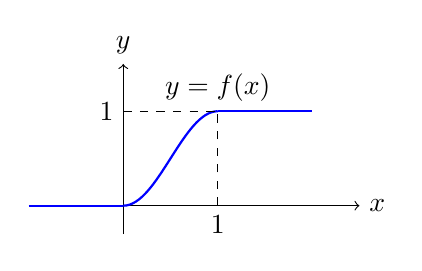
\begin{tikzpicture}[scale=1.2]
  % f(x)
  \draw[->] (-1,0) -- (2.5,0) node[right] {$x$};
  \draw[->] (0,-0.3) -- (0,1.5) node[above] {$y$};
  \draw[thick, blue] (-1,0) -- (0,0);
  \draw[thick, blue] (0,0) cos (0.5,0.5) sin (1,1);
  \draw[thick, blue] (1,1) -- (2,1);
  \node[above] at (1,1) {$y=f(x)$};
  \draw[dashed] (1,0) node[below] {$1$} -- (1,1);
  \draw[dashed] (0,1) node[left] {$1$} -- (1,1);
\end{tikzpicture}
\qquad
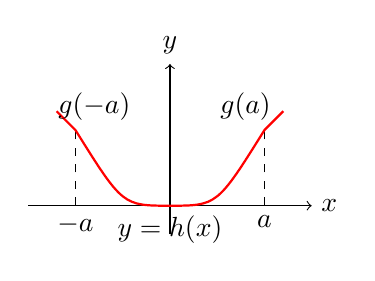
\begin{tikzpicture}[scale=1.2]
  % h(x)
  \draw[->] (-1.5,0) -- (1.5,0) node[right] {$x$};
  \draw[->] (0,-0.3) -- (0,1.5) node[above] {$y$};
  \draw[dashed] (-1,0) node[below] {$-a$} -- (-1,0.8);
  \draw[dashed] (1,0) node[below] {$a$} -- (1,0.8);
  \draw[thick, red] (-1.2,1) -- (-1,0.8) .. controls (-0.5,0) .. (0,0) .. controls (0.5,0) .. (1,0.8) -- (1.2,1);
  \node[above] at (0.8,0.8) {$g(a)$};
  \node[above] at (-0.8,0.8) {$g(-a)$};
  \node[below] at (0,0) {$y=h(x)$};
\end{tikzpicture}
\end{center}

(i) $h(x) = \begin{cases} g(x) f\left(\frac{x}{a}\right) & (0 \le x) \\ g(x) f\left(-\frac{x}{a}\right) & (x \le 0) \end{cases}$ が (イ), (ニ) を満たすことを示す. まず (ロ) から $h(0) = 0$ となって (ハ) を満たす. 次に (ニ) について,
$a < x$ の時 $f\left(\frac{x}{a}\right) = 1$ から $h(x) = g(x)$
$x < -a$ の時 $f\left(-\frac{x}{a}\right) = 1$ から $h(x) = g(x)$
となって (ニ) も満たす. 又 $g, f$ 共に微分可能だから $h(x)$ も $x \ne 0$ では微分可能である. ここで (イ) から $f'(0) = 0$ だから
\[
\lim_{x \to +0} \frac{h(x) - h(0)}{x} = \left. \left( g(x) f\left(\frac{x}{a}\right) \right)' \right|_{x=0} = \left. \left( g'(x) f\left(\frac{x}{a}\right) + \frac{1}{a} g(x) f'\left(\frac{x}{a}\right) \right) \right|_{x=0} = 0
\]
\[
\lim_{x \to -0} \frac{h(x) - h(0)}{x} = \left. \left( g(x) f\left(-\frac{x}{a}\right) \right)' \right|_{x=0} = \left. \left( g'(x) f\left(-\frac{x}{a}\right) - \frac{1}{a} g(x) f'\left(-\frac{x}{a}\right) \right) \right|_{x=0} = 0
\]
となって左右極限が一致し、$x=0$ でも $h(x)$ は微分可能. 以上からこの $h(x)$ は題意を満たす.
\[
h(x) = \begin{cases} g(x) f\left(\frac{x}{a}\right) & (0 \le x) \\ g(x) f\left(-\frac{x}{a}\right) & (x \le 0) \end{cases}
\]

\medskip
(ii) $f(x) = \begin{cases} 0 & (x \le 0) \\ 2x^2 & (0 \le x \le 1/2) \\ -2(x-1)^2 + 1 & (1/2 \le x \le 1) \\ 1 & (1 \le x) \end{cases}$ が (イ) を満たすことをしめす. この関数は全区間で連続である. 又 $x \ne 0, 1/2, 1$ では微分可能.

まず、$g(x) = 2x^2$, $h(x) = -2(x-1)^2 + 1$ とおく. $g'(x) = 4x, h'(x) = -4(x-1)$ であり、
\[
\lim_{x \to +0} f'(x) = g'(0) = 0 = \lim_{x \to -0} f'(x)
\]
\[
\lim_{x \to \frac{1}{2} - 0} f'(x) = h'\left(\frac{1}{2}\right) = 2 = g'\left(\frac{1}{2}\right) = \lim_{x \to \frac{1}{2} + 0} f'(x)
\]
\[
\lim_{x \to 1 - 0} f'(x) = h'(1) = 0 = \lim_{x \to 1 + 0} f'(x)
\]
から、$f(x)$ は $x = 0, 1/2, 1$ でも微分可能. 以上から示された.
\end{proof}

\newpage

\section*{第6問}

\begin{proof}[解]
$U_1 \dots 4n$ 個の赤 と $n$ 個の白\\
$U_2 \dots 2n$ 個の赤 と $3n$ 個の白

誤った判断を下すのは、「$U_1$ が手渡されて $U_2$ と判断する $\dots A$」か「$U_2$ が手渡されて $U_1$ と判断する $\dots B$」のいずれか.

\medskip
1° Aの時\\
$U_1$ から $(\text{赤}, \text{白}) = (1, 2), (0, 3)$ をとり出した時で 確率は
\[
\frac{2}{3} \times \frac{_{4n}\mathrm{C}_1 \cdot _n\mathrm{C}_2 + _n\mathrm{C}_3}{_{5n}\mathrm{C}_3}
\]
(すべての玉を区別し、そのうちから3つをとり出す $_{5n}\mathrm{C}_3$ 通りが同様に確からしい)

\medskip
2° Bの時\\
$U_2$ から $(\text{赤}, \text{白}) = (3, 0), (2, 1)$ をとり出した時で 確率は
\[
\frac{1}{3} \times \frac{_{2n}\mathrm{C}_3 + _{2n}\mathrm{C}_2 \cdot _{3n}\mathrm{C}_1}{_{5n}\mathrm{C}_3}
\]

\medskip
以上から
\[
P_n = \frac{1}{3 \cdot _{5n}\mathrm{C}_3} \left[ 2 \cdot _{4n}\mathrm{C}_1 \cdot _n\mathrm{C}_2 + 2 \cdot _n\mathrm{C}_3 + _{2n}\mathrm{C}_3 + _{2n}\mathrm{C}_2 \cdot _{3n}\mathrm{C}_1 \right]
\]
\[
= \frac{6}{15n(5n-1)(5n-2)} \cdot \frac{1}{6} \left[ 24 n^2(n-1) + n(n-1)(n-2) + 2n(2n-1)(2n-2) + 18n^2(2n-1) \right]
\]
\[
= \frac{1}{15} \cdot \frac{1}{(5 - \frac{1}{n})(5 - \frac{2}{n})} \left[ 24\left(1 - \frac{1}{n}\right) + \left(1 - \frac{1}{n}\right)\left(1 - \frac{2}{n}\right) + 2\left(2 - \frac{1}{n}\right)\left(2 - \frac{2}{n}\right) + 18\left(2 - \frac{1}{n}\right) \right]
\]
\[
\longrightarrow \frac{1}{15} \cdot \frac{1}{25} [ 24 + 1 + 8 + 36 ] = \frac{69}{375} \quad (n \to \infty)
\]
\end{proof}

\end{document}
